\chapter{Reinforcement Learning and Deep Neural Networks}
\label{ch:reinforcement_learning}

\begin{remark}{Outline}

\end{remark}

\section{Introduction}
\label{sec:rl_introduction}


\section{Markov Decision Processes}
\label{sec:mdps}

In order to develop and apply RL algorithms to optimal decision making problems, we need to formulate the problem in a specific framework: in RL this is done with Markov Decision Processes (MDPs). Throughout this thesis we will characterize MDPs, and the resulting RL concepts, by using the mathematical notation that was used by \citet{sutton2018reinforcement} in their seminal book about RL, although it is worth noting that within the literature, different formulations can be found to express the same kind of concepts \cite{busoniu2010reinforcement}.

We start by introducing the following elements:
\begin{itemize}
	\item A set of possible states $\mathcal{S}$, that can be visited by an agent while it is interacting with the MDP, where $s_t \in \mathcal{S}$ denotes the state being visited at time-step $t$.
	\item A set of possible actions $\mathcal{A}$ that are available to the agent when it is in a certain state, where $a_t \in \mathcal{A}(s_t)$ denotes the action that is performed by the agent in state $s$ at time-step $t$.
\item A transition function $\mathcal{P}:\matchal{S}\times\matchal{A}\times\matchal{S}\Rightarrow [0,1]$ that defines the probability for an agent to visit state $s_{t+1}$, based on its current state and the action which will be performed thereafter. This probability is then defined as $p(s_{t+1}|s_t, a_t)$.
\item A reward function $\mathcal{R}:\matchal{S}\times\matchal{A}\times\matchal{S}\Rightarrow \mathbb{R}$ which returns a reward signal $r_{t+1}$ when an agent performs action $a_t$ in state $s_t$ and transits to $s_{t+1}$.
\item A discount factor denoted as $\gamma \in [0,1]$.

\end{itemize}

Based on these concepts a MDP is then defined by the following tuple $<\mathcal{S}, \matchcal{A}, \matchal{P}, \mathcal{R}, \gamma>$ and is also commonly denoted in the RL literature as the \textbf{environment}. The way the agent interacts with this environment is defined by its \textbf{policy} $\pi$ defined as
\begin{equation}
	\pi(a|s) = \text{Pr}\; \{A_t = a | S_t = s\}, \; \text{for all}\; s \in \mathcal{S}\; \text{and}\; a\ \in \mathcal{A} 
\end{equation}
which maps each state to an action $\pi:\mathcal{S}\Rightarrow\mathcal{A}$.

The elements of a MDP allow us to properly model the dynamics of an agent interacting with its environment, an interaction which can be summarized as follows: at each time-step $t$ the environment provides the agent with a certain state $s_t$, the agent then performs action $a_t$ which results into the reward signal $r_{t+1}$. After performing such action the agent will enter into the new state $s_{t+1}$. This continuous interaction with the environment is also known as the Reinforcement Learning loop, and can technically be infinite. This is however never the case in practice, since we assume that an agent will eventually visit a state which only transits to itself (denoted as terminal), which will therefore stop the agent-environment interaction. We visually represent the Reinforcement Learning loop in Fig.\ref{fig:rl_loop}.

\begin{figure}[ht!]
\centering
  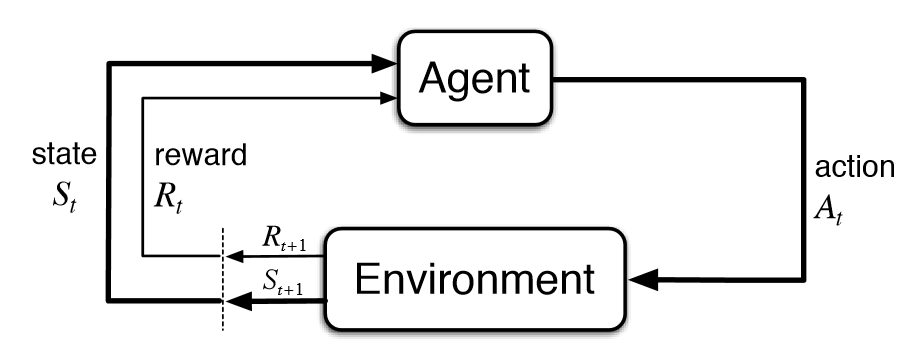
\includegraphics[width=10cm]{./Images/Chapter06/rl_loop.png}
  \caption{A visual representation of how an agent interacts with an environment as modeled by a Markov decision process. Figure taken from page 48 of the \citet{sutton2018reinforcement} textbook.}
  \label{fig:rl_loop}
\end{figure}



\section{Value Functions}


\section{Learning Value Functions}
\subsection{Monte Carlo Methods}
\subsection{Temporal Difference Learning}

\section{Function Approximators}
\subsection{Linear Functions}

\subsection{Deep Neural Networks}

\section{}
